\documentclass{standalone}
\usepackage{graphicx}	
\usepackage{amssymb, amsmath, amsthm}
\usepackage{color}

\usepackage{tikz}
\usetikzlibrary{intersections, backgrounds, math, decorations.pathreplacing}

\definecolor{light}{RGB}{220, 188, 188}
\definecolor{mid}{RGB}{185, 124, 124}
\definecolor{dark}{RGB}{143, 39, 39}
\definecolor{highlight}{RGB}{180, 31, 180}
\definecolor{darkteal}{RGB}{29, 79, 79}
\definecolor{darkolive}{RGB}{97, 123, 45}
\definecolor{gray10}{gray}{0.1}
\definecolor{gray20}{gray}{0.2}
\definecolor{gray30}{gray}{0.3}
\definecolor{gray40}{gray}{0.4}
\definecolor{gray60}{gray}{0.6}
\definecolor{gray70}{gray}{0.7}
\definecolor{gray80}{gray}{0.8}
\definecolor{gray90}{gray}{0.9}
\definecolor{gray95}{gray}{0.95}

\begin{document}

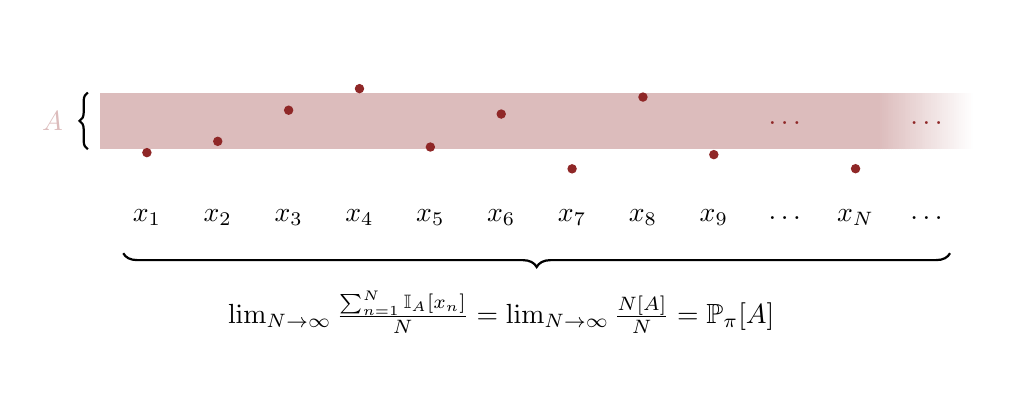
\begin{tikzpicture}[scale=0.3, thick]
  
\draw[white] (-2, -7) rectangle (39, 8);
  
\fill[light] (1, 2.9) rectangle(34, 5.3);

\foreach \delta in {1, 0.98, ..., 0} {
  \pgfmathsetmacro{\prop}{100 * \delta)};
  \colorlet{custom}{light!\prop!white};
  
  \draw[custom] ({34 + 4 * (1 - \delta)}, 2.9) -- +(0, 2.4);
}

\draw[decorate,decoration={brace,amplitude=3pt}] (0.5, 2.9) -- (0.5, 5.3);

\node[light] at (-1, 4.1) { $A$ };
 
\foreach \n in {1, 2, ..., 9} {
  \node at ({3 * \n}, 0) { $x_{\n}$ };
}
  
\foreach \x [count=\n] in {-1.2423804, -0.7652753,  0.5532082,  1.4655993, -1.0053407,  
                           0.3907344, -1.9280710,  1.1094778, -1.3272656} {
  \fill[dark] ({3 * \n}, \x + 4) circle (0.2);  
}
  
\node at (30, 0) { $\ldots$ };
\node[dark] at (30, 4) { $\ldots$ };

\node at (33, 0) { $x_{N}$ };
\fill[dark] (33, -1.92283385 + 4) circle (0.2);  

\node at (36, 0) { $\ldots$ };
\node[dark] at (36, 4) { $\ldots$ };

\draw[decorate,decoration={brace,amplitude=5pt,mirror}] (2, -1.5) -- (37, -1.5);

\node at (18, -4) { $\lim_{N \rightarrow \infty} \frac{ \sum_{n = 1}^{N} \mathbb{I}_{A}[ x_{n} ] }{ N } 
                     = \lim_{N \rightarrow \infty} \frac{ N[ A ] }{ N } = \mathbb{P}_{\pi}[A]$ };
  
\end{tikzpicture}

\end{document}  